\documentclass{beamer}
\usetheme{Pittsburgh}
\beamertemplatenavigationsymbolsempty


\usepackage{amsmath}
\usepackage{amssymb}
\usepackage{bm} % For bold math symbols
\usepackage{graphicx}
\usepackage{tikz}



\usepackage{subfig} % Changed from subfigure (deprecated)
\usepackage{multirow}
\usepackage{multicol}
\usepackage{color}
\usepackage{url}
\usepackage{hyperref}
\usepackage{listings}
\usepackage[noend]{algorithm}
\usepackage{physics} 

\usepackage{animate}

% add image path
\graphicspath{{Images/}}






\DeclareMathOperator{\argmin}{argmin}
\DeclareMathOperator{\argmax}{argmax}






\title{Weekly Updates\\
\tiny{Wednesday, 30/04/2025}}
\author{Andrea Bonifacio}
\date{}

\begin{document}

\begin{frame}
\titlepage
\end{frame}


\begin{frame}{What's Going On? - Key Issues}
    \begin{itemize}
        \item \textbf{Problem 1: Directions Aren't Perpendicular?}
        \begin{itemize}
            \item When we adjust different latent variables, the resulting shape changes don't seem independent.
            \item This doesn't match what we expected based on the reference paper.
        \end{itemize}
        \item \textbf{Problem 2: Weird Energy Results During Testing}
        \begin{itemize}
            \item We trained the model to find modes with low potential energy.
            \item However, when we test the model, the simple linear part alone often results in lower energy than the full model (linear + neural network). 
            \item Why could this happen?
            \begin{itemize}
                \item Is the model not generalizing well from training?
                \item Is there an issue with how we calculate energy for testing?
                \item Are our test cases too simple (showing little non-linear behavior)?
            \end{itemize}
        \end{itemize}
    \end{itemize}
\end{frame}

\begin{frame}
    \frametitle{Ensuring Orthogonal Total Directions}

    \begin{itemize}
        \item It seems that even if linear modes $\boldsymbol{\phi}_i$ are orthogonal and non-linear directions $\mathbf{e}_k^{\text{NN}}$ are orthogonal to linear modes, the total directions might not be orthogonal.
        % \item Specifically, for $i \neq j$:
        % \[
        %     (\mathbf{e}_i^{\text{total}})^T \mathbf{e}_j^{\text{total}} = (\mathbf{e}_i^{\text{NN}})^T \mathbf{e}_j^{\text{NN}}
        % \]
        \item \textbf{Implication:} To make the total directions $\mathbf{e}_i^{\text{total}}$ orthogonal, we likely need to enforce orthogonality between the non-linear directions themselves: $(\mathbf{e}_i^{\text{NN}})^T \mathbf{e}_j^{\text{NN}} = 0$ for $i \neq j$.
    \end{itemize}

\end{frame}

% \begin{frame}
%     \frametitle{Problem: Non-Orthogonal Total Directions (1/2)}

%     \begin{itemize}
%         \item Let the total displacement be $\mathbf{u}(\mathbf{z}) = \mathbf{l}(\mathbf{z}) + \mathbf{y}(\mathbf{z})$, where $\mathbf{l}(\mathbf{z}) = \mathbf{\Phi} \mathbf{z}$ (linear) and $\mathbf{y}(\mathbf{z}) = \text{NN}(\mathbf{z})$ (non-linear).
%         \item The direction vector associated with latent variable $z_i$ at $\mathbf{z}=\mathbf{0}$ is:
%         \[
%             \mathbf{e}_i^{\text{total}} = \frac{\partial \mathbf{u}}{\partial z_i} \bigg|_{\mathbf{z}=\mathbf{0}} = \underbrace{\boldsymbol{\phi}_i}_{\text{Linear direction}} + \underbrace{\frac{\partial \mathbf{y}}{\partial z_i}\bigg|_{\mathbf{z}=\mathbf{0}}}_{\mathbf{e}_i^{\text{NN}} \text{ (Non-linear direction)}}
%         \]
%         where $\boldsymbol{\phi}_i$ is the $i$-th column of $\mathbf{\Phi}$.

%         \item \textbf{Assumptions/Conditions:}
%         \begin{enumerate}
%             \item The linear modes $\boldsymbol{\phi}_i$ are orthogonal: $\boldsymbol{\phi}_i^T \boldsymbol{\phi}_j = 0$ for $i \neq j$.
%             \item We enforce that each non-linear direction $\mathbf{e}_k^{\text{NN}}$ is orthogonal to all linear modes $\boldsymbol{\phi}_m$: $(\mathbf{e}_k^{\text{NN}})^T \boldsymbol{\phi}_m = 0$ for all $k, m$.
%         \end{enumerate}

%         \item \textbf{Question:} Given (1) and (2), why is $\mathbf{e}_i^{\text{total}}$ not necessarily orthogonal to $\mathbf{e}_j^{\text{total}}$ when $i \neq j$?
%     \end{itemize}

% \end{frame}

% \begin{frame}
%     \frametitle{Analysis: Why Total Directions Aren't Orthogonal (2/3)}

%     \begin{itemize}
%         \item Recall: $\mathbf{e}_i^{\text{total}} = \boldsymbol{\phi}_i + \mathbf{e}_i^{\text{NN}}$
%         \item \textbf{Analysis:} Let's compute the dot product for $i \neq j$:
%         \begin{align*}
%             (\mathbf{e}_i^{\text{total}})^T \mathbf{e}_j^{\text{total}} &= (\boldsymbol{\phi}_i + \mathbf{e}_i^{\text{NN}})^T (\boldsymbol{\phi}_j + \mathbf{e}_j^{\text{NN}}) \\
%             &= \underbrace{\boldsymbol{\phi}_i^T \boldsymbol{\phi}_j}_{\substack{=0 \\ \text{(by assumption 1)}}} + \underbrace{\boldsymbol{\phi}_i^T \mathbf{e}_j^{\text{NN}}}_{\substack{=0 \\ \text{(by assumption 2)}}} \\
%             & \quad + \underbrace{(\mathbf{e}_i^{\text{NN}})^T \boldsymbol{\phi}_j}_{\substack{=0 \\ \text{(by assumption 2)}}} + (\mathbf{e}_i^{\text{NN}})^T \mathbf{e}_j^{\text{NN}} \\
%             &= (\mathbf{e}_i^{\text{NN}})^T \mathbf{e}_j^{\text{NN}}
%         \end{align*}
%     \end{itemize}
% \end{frame}

% \begin{frame}
%     \frametitle{Analysis: Why Total Directions Aren't Orthogonal (3/3)}

%     \begin{itemize}
%         \item From the previous slide, we found:
%         \[
%             (\mathbf{e}_i^{\text{total}})^T \mathbf{e}_j^{\text{total}} = (\mathbf{e}_i^{\text{NN}})^T \mathbf{e}_j^{\text{NN}} \quad \text{for } i \neq j
%         \]

%         \item \textbf{Conclusion:} The orthogonality of the total directions $(\mathbf{e}_i^{\text{total}})^T \mathbf{e}_j^{\text{total}} = 0$ holds if and only if the non-linear directions are orthogonal to each other: $(\mathbf{e}_i^{\text{NN}})^T \mathbf{e}_j^{\text{NN}} = 0$.
%         \item Our enforced condition (2) only ensures non-linear directions are orthogonal to linear modes, \textit{not} necessarily to other non-linear directions. Hence, the sum (total direction) is generally not orthogonal.
%     \end{itemize}

% \end{frame}

\begin{frame}
    \frametitle{Correlation of Latent Space}
    
    \begin{figure}
        \centering
        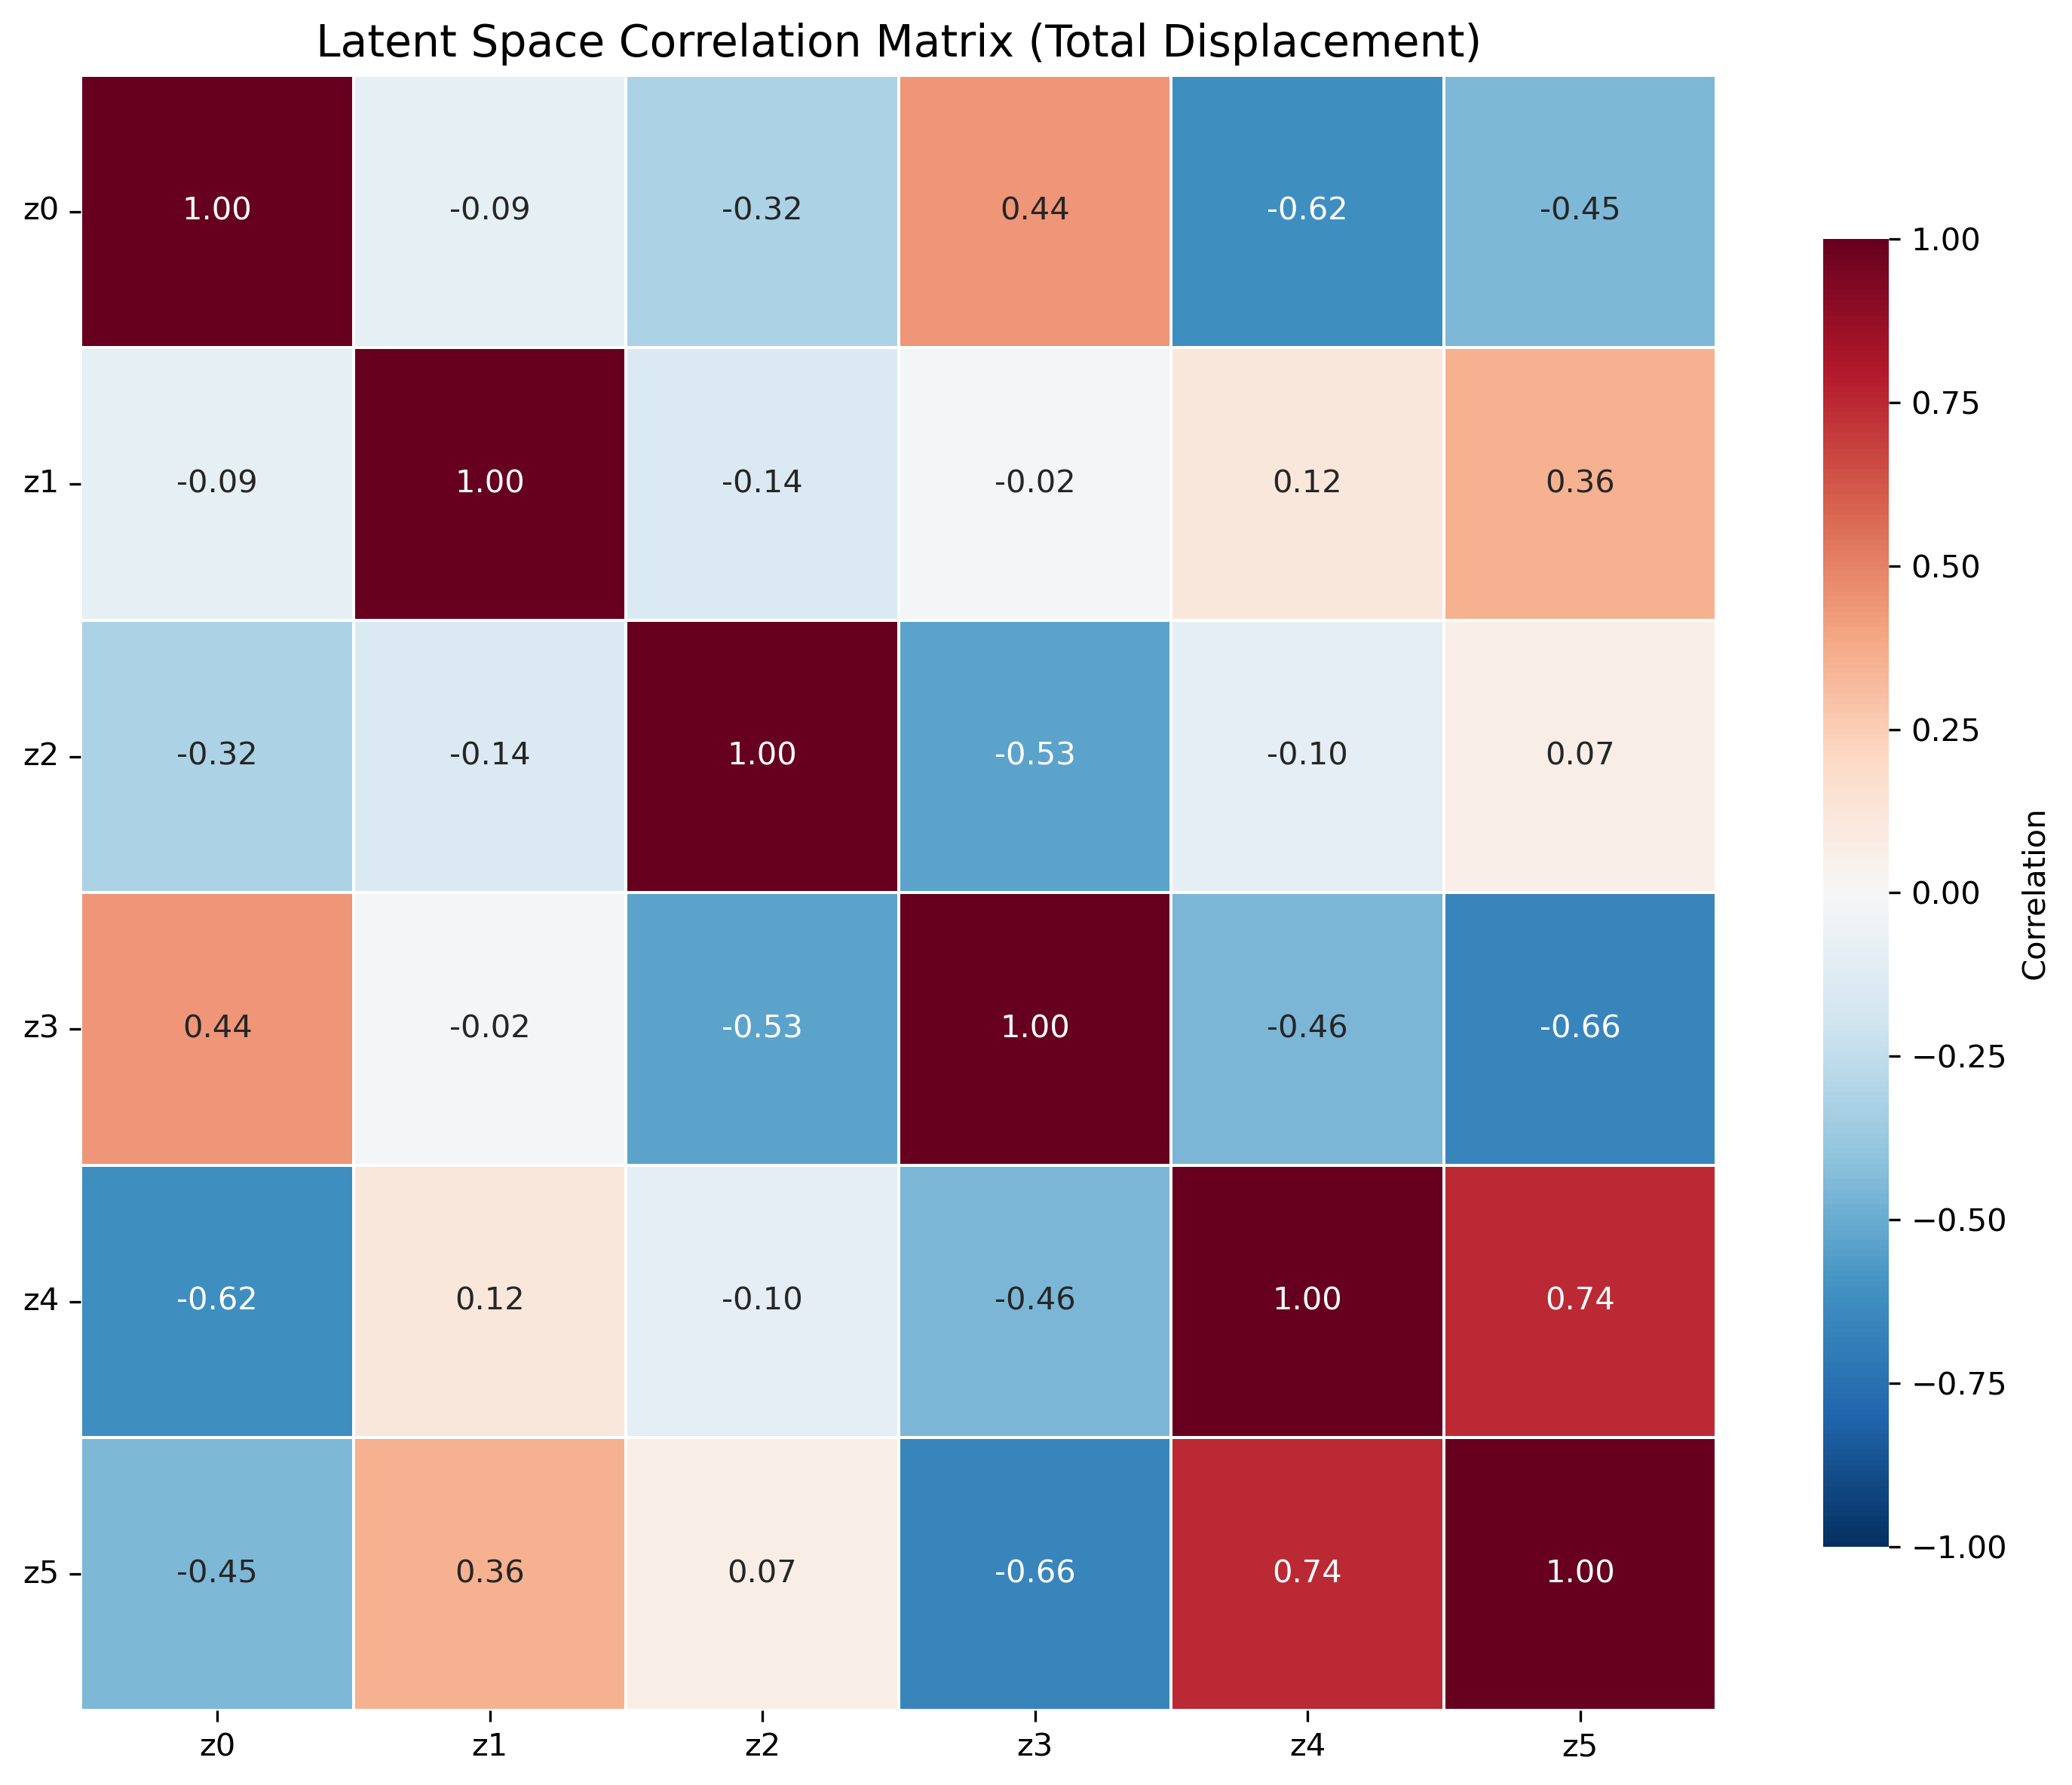
\includegraphics[width=0.7\textwidth]{Images/latent_correlations_total_total.png}
        \caption{Correlation of latent space.}
        \label{fig:latent_correlation}

    \end{figure}
\end{frame}








\begin{frame}
    \frametitle{Validation Static Case}
    
    \begin{itemize}
        \item The energy is computed for all the three cases: linear modes, neural network, and the reference solution using the energy calculator of the neural network.
        \item While during the training, the energy of the neural modes is much lower (100x) than the one of the linear modes, when validating the results, linear modes have a much lower energy.
        \item This could mean that the network is not generalizing well, or that my simulations are exhibiting very little nonlinear behavior. But I am preparing a simulation with a torque applied to the beam to see if I can get a more nonlinear behavior.
        \item I am trying to add a beam with a linear elasticity model in the simulations, to compare it with the result I obtain from linear modes, but at the moment it is buggy, so I did not include it.
    \end{itemize}
\end{frame}

\begin{frame}
    \frametitle{Energy results}
    
    \begin{figure}
        \centering
        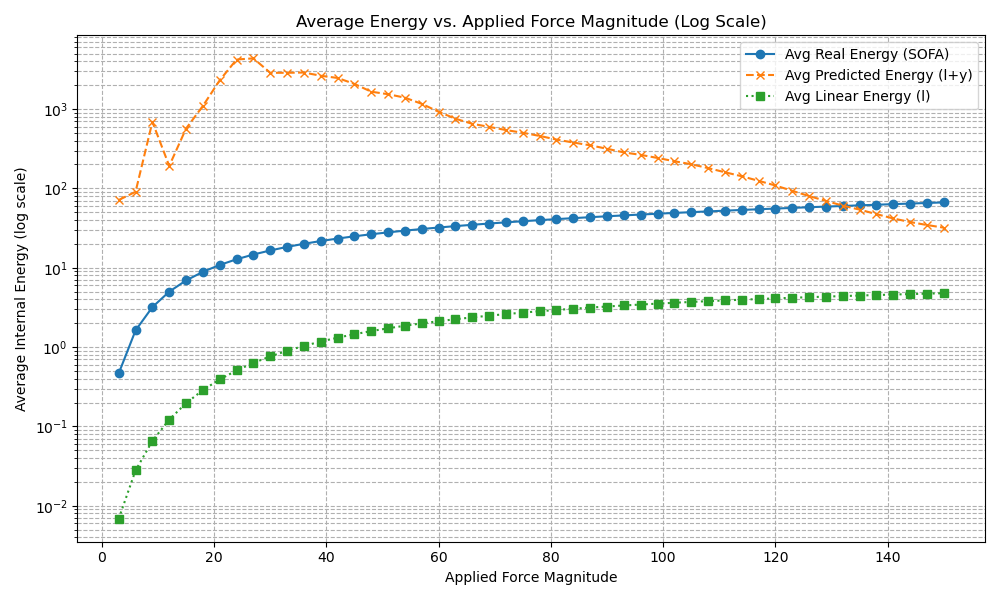
\includegraphics[width=0.8\textwidth]{Images/avg_energy_vs_force_log.png}
        \caption{Energy of various modes as a function of the applied force.}
        \label{fig:linear_correlation}

    \end{figure}
    \end{frame}
% Q&A
\begin{frame}
    \begin{center}
        \color{blue} \Huge{Questions?}
    \end{center}

\end{frame}
\end{document}

